\documentclass{ximera}

\newcommand{\RR}{\mathbb R}
\renewcommand{\d}{\,d}
\newcommand{\dd}[2][]{\frac{d #1}{d #2}}
\renewcommand{\l}{\ell}
\newcommand{\ddx}{\frac{d}{dx}}
\newcommand{\dfn}{\textbf}
\newcommand{\eval}[1]{\bigg[ #1 \bigg]}


\title[Dig-In:]{Slopes of tangent lines via limits} %% I don't know about this title

\begin{document}
\begin{abstract}
We compute the derivative by computing the limits of average growth %% I don't know about this absract
rates.
\end{abstract}
\maketitle


Suppose that $f(x)$ is a function.  It is often useful to know the
rate at which $f(x)$ changes. To give you a feeling why this is true,
consider the following:
\begin{itemize}
\item If $s(t)$ represents the displacement (position relative to an
  origin) of an object with respect to time, the rate of change gives
  the velocity of the object.
\item If $v(t)$ represents the velocity of an object with respect to
  time, the rate of change gives the acceleration of the object.
\item If $R(x)$ represents the revenue generated by selling $x$
  objects, the rate of change gives us the \textit{marginal revenue},
  meaning the additional revenue generated by selling one additional
  unit. Note, there is an implicit assumption that $x$ is quite large
  compared to $1$.
\item If $C(x)$ represents the cost to produce $x$ objects, the rate
  of change gives us the \textit{marginal cost}, meaning the
  additional cost generated by selling one additional unit. Again,
  there is an implicit assumption that $x$ is quite large compared to
  $1$.
\item If $P(x)$ represents the profit gained by selling $x$ objects,
  the rate of change gives us the \textit{marginal profit}, meaning
  the additional cost generated by selling one additional unit. Again,
  there is an implicit assumption that $x$ is quite large compared to
  $1$.
\item The rate of change of a function can help us approximate a
  complicated function with a simple function.
\item The rate of change of a function can be used to help us solve
  equations that we would not be able to solve via other methods.
\end{itemize}

\begin{xarmaBoost}
What other examples can you find where one is interested in a ``rate
of change?''
\begin{freeResponse}
\end{freeResponse}
\end{xarmaBoost}

\section{From average velocity to instantaneous velocity}

%%
%% I'm still not totally happy with this section
%%

Perhaps the most concrete example of a ``rate of change'' that we are
interested in is the first example above:
\begin{quote}
  If $s(t)$ represents the displacement (position relative to an origin)
  of an object with respect to time, the rate of change gives the
  velocity of the object.
\end{quote}
When one computes average velocity, we look at 
\[
\frac{\text{change in displacement}}{\text{change in time}}.
\]
To obtain the (instantaneous) velocity, we want the change in time to
``go to'' zero. By this point we should know that ``go to'' is a
buzz-word for a \textit{limit}. The change in time is often given as
an interval, by something like
\[
I = [a, a+h].
\]
However, intervals must always be written 
\[
[a,b]
\]
where $a < b$. Given $I = [a, a+h]$, we see that $h$ cannot be
negative, or else it violates the notation for intervals. Hence, if we
want smaller, and smaller, intervals, we write
\[
I_h = 
\begin{cases}
  [a+h,a]  & \text{if $-1<h<0$}, \\ %% note this is MORE correct than std books
  [a,a+h]  & \text{if $0<h<1$}.     %% in the content section, we can explain this in detail
\end{cases}
\]
Regardless of the value of $h$, the average velocity is computed by
\[
\frac{\text{change in displacement}}{\text{change in time}} =
\frac{s(t+h)-s(t)}{h}.
\]

Let's put this together by working an example.

\begin{example}
The \textit{MOOCulus Team} recently took a road trip from Columbus
Ohio to Urbana-Champaign Illinois in the \textit{MOOCulus-Mobile}. The
position of the MOOCulus-Mobile is roughly modeled by
\[
s(t) = 36t^2 - 4.8t^3 \qquad\text{(miles West of Columbus)} %% note the model is wrong
\]
on the interval $[0,5]$, where $t$ is measured in hours. The average
velocity on the interval $[0,5]$ is \answer{60} miles per hour. On the
other hand, consider the interval
\[
I_h = 
\begin{cases}
  [1+h,1]  & \text{if $-1<h<0$}, \\ %% note this is MORE correct than std books
  [1,1+h]  & \text{if $0<h<1$}.     %% in the content section, we can explain this in detail
\end{cases}
\]
When $h = 0.1$, the average velocity is \answer{59.712}. On the other
hand, when $h=-0.1$, the average velocity is \answer{55.392}.
\end{example}

Now let's change gears a bit. Displacement and velocity are good
metaphors for concepts in calculus. However, another powerful
metaphor comes from geometry, and this metaphor is too important to
postpone any longer.


\section{From slopes of secant lines to slopes of tangent lines}

You've been computing average rates of change for a while now, the
computation is simply
\[
\frac{\text{change in the function}}{\text{change in the input to the
    function}}.
\]
However, the question remains: Given a function that represents an
amount, how exactly does one find the function that will give the
instantaneous rate of change? Recall that the instantaneous rate of change
of a line is the slope of the line.  Hence the instantaneous rate of
change of a function is the slope of the tangent line. For now,
consider the following informal definition of a \textit{tangent line}:
\begin{quote}\index{tangent line}
Given a function $f(x)$, if one can ``zoom in''
on $f(x)$ sufficiently so that $f(x)$ seems to be a straight line,
then that line is the \dfn{tangent line} to $f(x)$ at the point
determined by $x$.
\end{quote}
We illustrate this informal definition with the following diagram:
\begin{image}
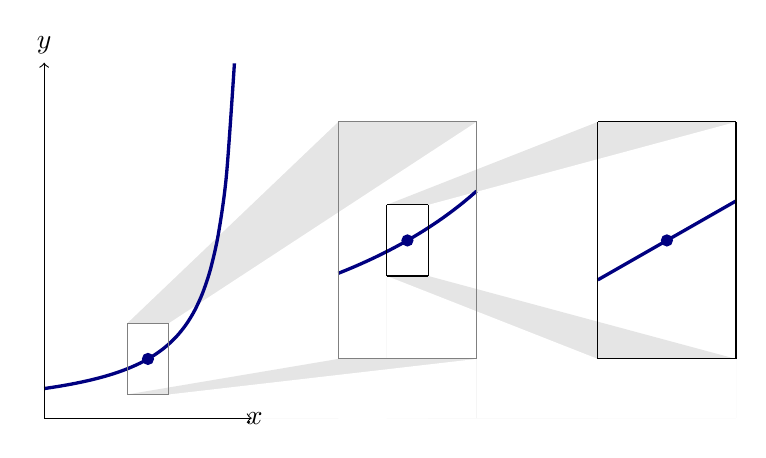
\begin{tikzpicture}
  \colorlet{penColor}{blue!50!black}
  \colorlet{penColor2}{red!50!black}
  \colorlet{textColor}{black}
  \colorlet{background}{white}
	\begin{axis}[
            domain=0:6, range=0:7,
            ymin=-.2,ymax=7,
            width=\textwidth,
            height=7cm, %% Hard coded height! Moreover this effects the aspect ratio of the zoom--sort of BAD
            axis lines=none,
          ]   
          \addplot [draw=none, fill=textColor!10!background] plot coordinates {(.8,1.6) (2.834,5)} \closedcycle; %% zoom fill
          \addplot [draw=none, fill=textColor!10!background] plot coordinates {(2.834,5) (4.166,5)} \closedcycle; %% zoom fill
          \addplot [draw=none, fill=background] plot coordinates {(1.2,1.6) (4.166,5)} \closedcycle; %% zoom fill
          \addplot [draw=none, fill=background] plot coordinates {(.8,1.6) (1.2,1.6)} \closedcycle; %% zoom fill

          \addplot [draw=none, fill=textColor!10!background] plot coordinates {(3.3,3.6) (5.334,5)} \closedcycle; %% zoom fill
          \addplot [draw=none, fill=textColor!10!background] plot coordinates {(5.334,5) (6.666,5)} \closedcycle; %% zoom fill
          \addplot [draw=none, fill=background] plot coordinates {(3.7,3.6) (6.666,5)} \closedcycle; %% zoom fill
          \addplot [draw=none, fill=background] plot coordinates {(3.3,3.6) (3.7,3.6)} \closedcycle; %% zoom fill
          
          \addplot [draw=none, fill=textColor!10!background] plot coordinates {(3.7,2.4) (6.666,1)} \closedcycle; %% zoom fill
          \addplot [draw=none, fill=textColor!10!background] plot coordinates {(3.3,2.4) (3.7,2.4)} \closedcycle; %% zoom fill
          \addplot [draw=none, fill=background] plot coordinates {(3.3,2.4) (5.334,1)} \closedcycle; %% zoom fill          
          \addplot [draw=none, fill=background] plot coordinates {(5.334,1) (6.666,1)} \closedcycle; %% zoom fill
          

          \addplot [draw=none, fill=textColor!10!background] plot coordinates {(.8,.4) (2.834,1)} \closedcycle; %% zoom fill
          \addplot [draw=none, fill=textColor!10!background] plot coordinates {(2.834,1) (4.166,1)} \closedcycle; %% zoom fill
          \addplot [draw=none, fill=background] plot coordinates {(1.2,.4) (4.166,1)} \closedcycle; %% zoom fill
          \addplot [draw=none, fill=background] plot coordinates {(.8,.4) (1.2,.4)} \closedcycle; %% zoom fill

          \addplot[very thick,penColor, smooth,domain=(0:1.833)] {-1/(x-2)};
          \addplot[very thick,penColor, smooth,domain=(2.834:4.166)] {3.333/(2.050-.3*x)-0.333}; %% 2.5 to 4.333
          %\addplot[very thick,penColor, smooth,domain=(5.334:6.666)] {11.11/(1.540-.09*x)-8.109}; %% 5 to 6.833
          \addplot[very thick,penColor, smooth,domain=(5.334:6.666)] {x-3}; %% 5 to 6.833
          
          \addplot[color=penColor,fill=penColor,only marks,mark=*] coordinates{(1,1)};  %% point to be zoomed
          \addplot[color=penColor,fill=penColor,only marks,mark=*] coordinates{(3.5,3)};  %% zoomed pt 1
          \addplot[color=penColor,fill=penColor,only marks,mark=*] coordinates{(6,3)};  %% zoomed pt 2

          \addplot [->,textColor] plot coordinates {(0,0) (0,6)}; %% axis
          \addplot [->,textColor] plot coordinates {(0,0) (2,0)}; %% axis
          
          \addplot [textColor!50!background] plot coordinates {(.8,.4) (.8,1.6)}; %% box around pt
          \addplot [textColor!50!background] plot coordinates {(1.2,.4) (1.2,1.6)}; %% box around pt
          \addplot [textColor!50!background] plot coordinates {(.8,1.6) (1.2,1.6)}; %% box around pt
          \addplot [textColor!50!background] plot coordinates {(.8,.4) (1.2,.4)}; %% box around pt
          
          \addplot [textColor!50!background] plot coordinates {(2.834,1) (2.834,5)}; %% zoomed box 1
          \addplot [textColor!50!background] plot coordinates {(4.166,1) (4.166,5)}; %% zoomed box 1
          \addplot [textColor!50!background] plot coordinates {(2.834,1) (4.166,1)}; %% zoomed box 1
          \addplot [textColor!50!background] plot coordinates {(2.834,5) (4.166,5)}; %% zoomed box 1

          \addplot [textColor] plot coordinates {(3.3,2.4) (3.3,3.6)}; %% box around zoomed pt
          \addplot [textColor] plot coordinates {(3.7,2.4) (3.7,3.6)}; %% box around zoomed pt
          \addplot [textColor] plot coordinates {(3.3,3.6) (3.7,3.6)}; %% box around zoomed pt
          \addplot [textColor] plot coordinates {(3.3,2.4) (3.7,2.4)}; %% box around zoomed pt

          \addplot [textColor] plot coordinates {(5.334,1) (5.334,5)}; %% zoomed box 2
          \addplot [textColor] plot coordinates {(6.666,1) (6.666,5)}; %% zoomed box 2
          \addplot [textColor] plot coordinates {(5.334,1) (6.666,1)}; %% zoomed box 2
          \addplot [textColor] plot coordinates {(5.334,5) (6.666,5)}; %% zoomed box 2

          \node at (axis cs:2.2,0) [anchor=east] {$x$};
          \node at (axis cs:0,6.6) [anchor=north] {$y$};
        \end{axis}
\end{tikzpicture}
%% \caption{Given a function $f(x)$, if one can ``zoom in''
%% on $f(x)$ sufficiently so that $f(x)$ seems to be a straight line,
%% then that line is the \textbf{tangent line} to $f(x)$ at the point
%% determined by $x$.}
%% \label{figure:informal-tangent}
\end{image}



The \textit{derivative} of a function $f(x)$ at $x$, is the instantaneous
rate of change, and hence is the slope of the tangent line at $x$. To
find the slope of this line, we consider \textit{secant} lines, lines
that locally intersect the curve at two points.  The slope of any
secant line that passes through the points $(x,f(x))$ and $(x+h,
f(x+h))$ is given by
\[
\frac{\Delta y}{\Delta x}=\frac{f(x+h) -f(x)}{(x+h)-x} =
\frac{f(x+h)-f(x)}{h}.
\]
%see Figure~\ref{figure:limit-dfn}. 
This leads to the \textit{limit definition of the derivative}:

%\begin{definitionOfTheDerivative}\index{limit!definition of the derivative}\index{derivative!limit definition}
\begin{definition}
The \dfn{derivative} of $f(x)$ is the function
\[
\ddx f(x) = \lim_{h\to 0} \frac{f(x+h) - f(x)}{h}.
\]
If this limit does not exist for a given value of $x$, then $f(x)$ is
not \dfn{differentiable} at $x$.
\end{definition}
%\end{definitionOfTheDerivative}
%\begin{marginfigure}[-1.75in]
\begin{image}
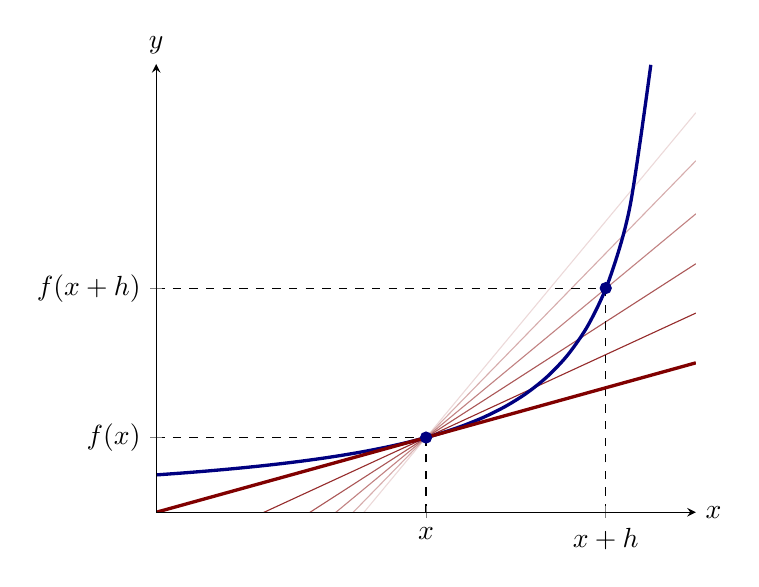
\begin{tikzpicture}
  \colorlet{penColor}{blue!50!black}
  \colorlet{penColor2}{red!50!black}
  \colorlet{textColor}{black}
  \colorlet{background}{white}  
	\begin{axis}[
            domain=0:2, range=0:6,ymax=6,ymin=0,
            axis lines =left, xlabel=$x$, ylabel=$y$,
            every axis y label/.style={at=(current axis.above origin),anchor=south},
            every axis x label/.style={at=(current axis.right of origin),anchor=west},
            xtick={1,1.666}, ytick={1,3},
            xticklabels={$x$,$x+h$}, yticklabels={$f(x)$,$f(x+h)$},
            axis on top,
          ]         
          \addplot [penColor2!15!background, domain=(0:2)] {-3.348+4.348*x};
          \addplot [penColor2!32!background, domain=(0:2)] {-2.704+3.704*x};
          \addplot [penColor2!49!background, domain=(0:2)] {-1.994+2.994*x};         
          \addplot [penColor2!66!background, domain=(0:2)] {-1.326+2.326*x}; 
          \addplot [penColor2!83!background, domain=(0:2)] {-0.666+1.666*x};
	  \addplot [textColor,dashed] plot coordinates {(1,0) (1,1)};
          \addplot [textColor,dashed] plot coordinates {(0,1) (1,1)};
          \addplot [textColor,dashed] plot coordinates {(0,3) (1.666,3)};
          \addplot [textColor,dashed] plot coordinates {(1.666,0) (1.666,3)};
          \addplot [very thick,penColor, smooth,domain=(0:1.833)] {-1/(x-2)};
          \addplot[color=penColor,fill=penColor,only marks,mark=*] coordinates{(1.666,3)};  %% closed hole          
          \addplot[color=penColor,fill=penColor,only marks,mark=*] coordinates{(1,1)};  %% closed hole          
          \addplot [very thick,penColor2, smooth,domain=(0:2)] {x};
        \end{axis}
\end{tikzpicture}
\end{image}
%% \caption{Tangent lines can be found as the limit of secant lines. The slope of the tangent line is given by
%% $\lim_{h\to 0} \frac{f(x+h) - f(x)}{h}.$}
%%  \label{figure:limit-dfn}
%% \end{marginfigure}

%\break



\begin{question} 

%% How do we write this question? I want to get both standard dfns of
%% the derivative out here, along with negations of the numerator and
%% denominator. How is a good questions constructed here?

Consider the following limits:
\begin{enumerate}
\item $\lim_{x\to a} \frac{f(x)-f(a)}{x-a}$\\
\item $\lim_{x\to a} \frac{f(a)-f(x)}{a-x}$\\
\item FIX THIS
\end{enumerate}
Can you explain why each of the limits above are also equivalent
definitions of the derivative?
\end{question}

\begin{definition}\index{derivative!notation}
There are several different notations for the derivative, we'll mainly
use
\[
\ddx f(x) = f'(x).
\]
If one is working with a function of a variable other than $x$, say $t$ we write
\[
\dd{t} f(t) = f'(t).
\]
However, if $y = f(x)$, $\dd[y]{x}$, $\dot{y}$, and $D_x f(x)$ are
also used.
\end{definition}

Now we will give a number of examples, starting with a basic example.

\begin{example}
Compute 
\[
\ddx (x^3 + 1).
\]
Start by writing out the limit definition of the derivative where
$f(x) = x^3+1$.
\begin{hint}
\[
\ddx f(x) = \lim_{h\to 0}\frac{(x+h)^3 + 1 - (x^3 +1)}{h}
\]
\end{hint}
Now expand the numerator of the fraction.
\begin{hint}
\[
\ddx f(x) = \lim_{h\to 0}\frac{x^3+3x^2h+3xh^2 + h^3 + 1 - x^3 -1}{h}
\]
\end{hint}
Now combine like-terms.
\begin{hint}
\[
\ddx f(x) = \lim_{h\to 0}\frac{3x^2h+3xh^2 + h^3}{h}
\]
\end{hint}
Factor an $h$ from every term in the numerator.
\begin{hint}
\[
\ddx f(x) = \lim_{h\to 0}\frac{h(3x^2+3xh + h^2)}{h}
\]
\end{hint}
Cancel $h$ from the numerator and denominator.
\begin{hint}
\[
\ddx f(x) = \lim_{h\to 0} \left(3x^2+3xh + h^2\right)
\]
\end{hint}
Take the limit as $h$ goes to $0$. 
\begin{hint}
\[
\ddx f(x) = 3x^2
\]
\end{hint}
%% Using the definition of the derivative,
%% \begin{align*}
%% \ddx f(x) &= \lim_{h\to 0}\frac{(x+h)^3 + 1 - (x^3 +1)}{h}\\
%% &= \lim_{h\to 0}\frac{x^3+3x^2h+3xh^2 + h^3 + 1 - x^3 -1}{h}\\
%% &= \lim_{h\to 0}\frac{3x^2h+3xh^2 + h^3}{h}\\
%% &= \lim_{h\to 0}(3x^2+3xh + h^2)\\
%% &= 3x^2.
%% \end{align*}
For your viewing pleasure, we have supplied a plot of both $f(x)$ and
$f'(x)$:
\begin{image}
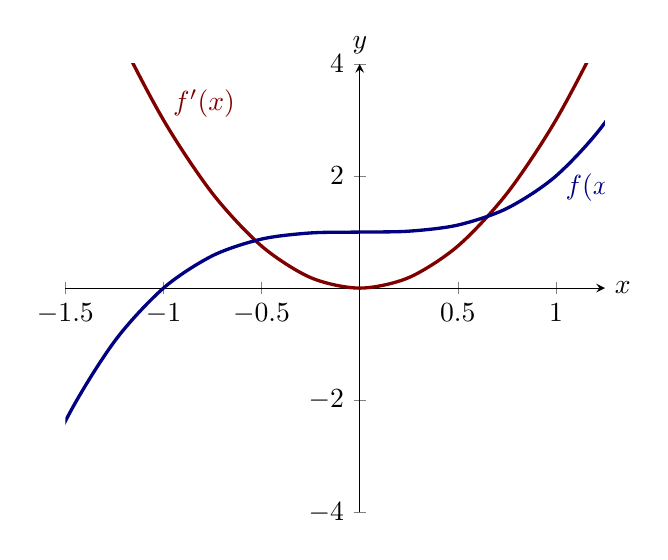
\begin{tikzpicture}
  \colorlet{background}{white}
  \colorlet{textColor}{black}
  \colorlet{penColor}{blue!50!black}
  \colorlet{penColor2}{red!50!black}
	\begin{axis}[
            domain=-3:3,
            ymax=4,
            ymin=-4,
            %samples=100,
            axis lines =middle, xlabel=$x$, ylabel=$y$,
            every axis y label/.style={at=(current axis.above origin),anchor=south},
            every axis x label/.style={at=(current axis.right of origin),anchor=west}
          ]
          \addplot [very thick, penColor2, smooth,domain=(-3:3)] {3*x^2};
          \addplot [very thick, penColor, smooth,domain=(-3:3)] {x^3+1};
          \node at (axis cs:1,1.8) [anchor=west] {\color{penColor}$f(x)$};  
          \node at (axis cs:-1,3.3) [anchor=west] {\color{penColor2}$f'(x)$};
        \end{axis}
\end{tikzpicture}
%\caption{A plot of $f(x) = x^3+1$ and $f'(x) = 3x^2$.}
%\label{figure:x^3+1}
\end{image}
\end{example}




\end{document}

%% I've stopped here for now. 





Next we will consider the derivative a function that is not continuous
on $\RR$.


\begin{example}
Compute
\[
\dd t \frac{1}{t}.
\]
\end{example}

\begin{solution}
Using the definition of the derivative,
\begin{align*}
\dd{t}\frac{1}{t}&=\lim_{ h\to0}\frac{\frac{1}{t+ h} - \frac{1}{t}}{h} \\
&=\lim_{h\to0}\frac{\frac{t}{t(t+ h)} - \frac{t+ h}{t(t+ h)}}{h} \\
&=\lim_{h\to0}\frac{\frac{t-(t+ h)}{t(t+ h)}}{h} \\
&=\lim_{h\to0}\frac{t-t- h}{t(t+ h) h} \\
&=\lim_{h\to0}\frac{- h}{t(t+ h) h} \\
&=\lim_{h\to0}\frac{-1}{t(t+ h)}\\
&=\frac{-1}{t^2}.
\end{align*}
This function is differentiable at all real numbers except for $t=0$, see Figure~\ref{figure:plot1/x}.
\end{solution}
\begin{marginfigure}
\begin{tikzpicture}
	\begin{axis}[
            domain=-3:3,
            ymax=4,
            ymin=-4,
            samples=100,
            axis lines =middle, xlabel=$t$, ylabel=$y$,
            every axis y label/.style={at=(current axis.above origin),anchor=south},
            every axis x label/.style={at=(current axis.right of origin),anchor=west}
          ]
          \addplot [very thick, penColor2, smooth,domain=(-3:-.1)] {-1/x^2};
          \addplot [very thick, penColor2, smooth,domain=(.1:3)] {-1/x^2};
	  \addplot [very thick, penColor, smooth,domain=(-3:-.1)] {1/x};
          \addplot [very thick, penColor, smooth,domain=(.1:3)] {1/x};
          \node at (axis cs:1,1.3) [anchor=west] {\color{penColor}$f(t)$}; 
          \node at (axis cs:1,-1.1) [anchor=west] {\color{penColor2}$f'(t)$};
        \end{axis}
\end{tikzpicture}
\caption{A plot of $f(t) = \frac{1}{t}$ and $f'(t) = \frac{-1}{t^2}$.}
\label{figure:plot1/x}
\end{marginfigure}

Let us now answer the following question: MOOCulus MOBILE




%% Perhaps a split should be made here!!



As you may have guessed, there is some connection to continuity and
differentiability. 



\begin{mainTheorem}[Differentiability Implies Continuity]\label{theorem:diff-cont}
If $f(x)$ is a differentiable function at $x = a$, then $f(x)$ is
continuous at $x=a$.
\end{mainTheorem}

\begin{proof}
We want to show that $f(x)$ is continuous at $x=a$, hence we must show that 
\[
\lim_{x\to a} f(x) = f(a).
\]
Consider
\begin{align*}
\lim_{x\to a} \left(f(x) - f(a)\right) &= \lim_{x\to a} \left((x-a)\frac{f(x) - f(a)}{x-a}\right) &\text{Multiply and divide by $(x-a)$.} \\
&= \lim_{h\to 0} h \cdot \frac{f(a+h) - f(a)}{h} &\text{Set $x = a+h$.} \\
&= \left(\lim_{h\to 0} h\right) \left(\lim_{h\to 0}\frac{f(a+h) - f(a)}{h}\right) &\text{Limit Law.} \\
&= 0\cdot f'(a) = 0.
\end{align*}
Since 
\[
\lim_{x\to a}\left(f(x) - f(a)\right) = 0 
\]
we see that $\lim_{x\to a} f(x) = f(a)$, and so $f(x)$ is continuous.
\end{proof}

This theorem is often written as its contrapositive:
\begin{quote}
If $f(x)$ is not continuous at $x=a$, then $f(x)$ is not
differentiable at $x=a$.
\end{quote}


Let's see a function that is continuous whose derivative does not
exist everywhere.


\begin{example}
Compute 
\[
\ddx |x|.
\]
\end{example}
\begin{marginfigure}
\begin{tikzpicture}
	\begin{axis}[
            domain=-3:3,
            ymax=3,
            ymin=-2,
            samples=100,
            axis lines =middle, xlabel=$x$, ylabel=$y$,
            every axis y label/.style={at=(current axis.above origin),anchor=south},
            every axis x label/.style={at=(current axis.right of origin),anchor=west}
          ]
          \addplot [very thick, penColor2, smooth,domain=(0:3)] {1};
          \addplot [very thick, penColor2, smooth,domain=(-3:0)] {-1};
          \addplot [very thick, penColor, smooth] {abs(x)};
          \node at (axis cs:1,1.7) [anchor=west] {\color{penColor}$f(t)$}; 
          \node at (axis cs:-1,-1.5) [anchor=south] {\color{penColor2}$f'(t)$};
          \addplot[color=penColor2,fill=background,only marks,mark=*] coordinates{(0,1)};  %% open hole
          \addplot[color=penColor2,fill=background,only marks,mark=*] coordinates{(0,-1)};  %% open hole
        \end{axis}
\end{tikzpicture}
\caption[A plot of $f(x) = |x|$ and its derivative.]{A plot of $f(x) = |x|$ and \[
f'(x) = \begin{cases}
1 &\text{if $x>0$,}\\
-1 &\text{if $x<0$.}
\end{cases}\]
}
\label{figure:plot-abs}
\end{marginfigure}
\begin{solution}
Using the definition of the derivative,
\[
\ddx |x| = \lim_{h\to0}\frac{|x+h| -|x|}{h}.
\]
If $x$ is positive we may assume that $x$ is larger than $h$, as we are
taking the limit as $h$ goes to $0$,
\begin{align*}
\lim_{h\to0}\frac{|x+h| -|x|}{h} &= \lim_{h\to0}\frac{x+h -x}{h}\\
&= \lim_{h\to0}\frac{h}{h}\\
&= 1.
\end{align*}
If $x$ is negative we may assume that $|x|$ is larger than $h$, as we are taking
the limit as $h$ goes to $0$,
\begin{align*}
\lim_{h\to0}\frac{|x+h| -|x|}{h} &= \lim_{h\to0}\frac{-x-h +x}{h}\\
&= \lim_{h\to0}\frac{-h}{h}\\
&= -1.
\end{align*}
However we still have one case left, when $x=0$. In this situation, we
must consider the one-sided limits:
\[
\lim_{h\to0+}\frac{|x+h| -|x|}{h}\qquad\text{and}\qquad \lim_{h\to0-}\frac{|x+h| -|x|}{h}.
\]
In the first case, 
\begin{align*}
\lim_{h\to0+}\frac{|x+h| -|x|}{h} &= \lim_{h\to 0+}\frac{0+h - 0}{h}\\
&= \lim_{h\to 0+}\frac{h}{h}\\
&=1.
\end{align*}
On the other hand
\begin{align*}
\lim_{h\to0-}\frac{|x+h| -|x|}{h} &= \lim_{h\to 0-}\frac{|0+h| - 0}{h}\\
&= \lim_{h\to 0-}\frac{|h|}{h}\\
&=-1.
\end{align*}
Hence we see that the derivative is
\[
f'(x) = 
\begin{cases}
1 &\text{if $x>0$,}\\
-1 &\text{if $x<0$.}
\end{cases}
\]
Note this function is undefined at $0$, see Figure~\ref{figure:plot-abs}. 
\end{solution}


Thus from Theorem~\ref{theorem:diff-cont}, we see that all
differentiable functions on $\RR$ are continuous on $\RR$. Nevertheless
as the previous example shows, there are continuous functions on $\RR$
that are not differentiable on $\RR$.






\end{document}
